\documentclass[12pt,francais]{beamer} 

\usepackage{multicol} %columnes
\usepackage{colortbl}
\usepackage{graphicx}
%\usepackage{amsmath}
%\usepackage{amsfonts}
%\usepackage{amssymb}
\usepackage{multimedia}
\usepackage[utf8]{inputenc}
\usepackage[T1]{fontenc}
\usepackage{lmodern}
\usepackage[francais]{babel}
\usepackage{bookman}
\usepackage{listings}
\usepackage{multicol}

\newcommand{\ble}[0] {$\bullet$ \space}
\setbeamertemplate{itemize item}[ball]
%\setbeamercolor{separation line}{use=structure,bg=structure.fg!10!bg} % ligne de séparation

%\useoutertheme[footline=institutetitle]{miniframes} % ligne de sous section + ligne du bas


\useinnertheme{rounded} % blocks arondis
\usecolortheme{rose} %permet les cadre autour des blocks
\setbeamertemplate{blocks}[rounded][shadow=true] % ombre block
\useoutertheme{smoothbars}
\useoutertheme{miniframes} % ligne de sous section
\setbeamertemplate{frametitle}[default][center] % centrer le titre
\DeclareOptionBeamer{subsection}[false]{\csname beamer@theme@subsection#1\endcsname}
\setbeamercolor{section in head/foot}{use=structure,bg=structure.fg!25!bg} % permet dégradé
\AtBeginDocument{%permet le dégradé en haut 
        {%
                \usebeamercolor{section in head/foot}
        }
        \pgfdeclareverticalshading{beamer@headfade}{\paperwidth}
        {%
                color(0cm)=(bg);
                color(1.25cm)=(section in head/foot.bg)%
        }
        \setbeamercolor{section in head/foot}{bg=}
}
\addtoheadtemplate{\pgfuseshading{beamer@headfade}\vskip-1.25cm}{} % dégradé
\beamertemplatedotitem
\DeclareOptionBeamer{compress}{\beamer@compresstrue} % ??
\ProcessOptionsBeamer % ??
\setbeamertemplate{navigation symbols}{} % suppression des symbols de nav
% ajout de la barre du bas
\setbeamertemplate{footline}{%
        \leavevmode%
        \hbox{\hspace*{-0.06cm}
        \begin{beamercolorbox}[wd=0.30\paperwidth,ht=2.25ex,dp=1ex,left]{author in head/foot}%
                \usebeamerfont{author in head/foot} LIP6 - SoC - Alsoc
        \end{beamercolorbox}%
        \begin{beamercolorbox}[wd=0.48\paperwidth,ht=2.25ex,dp=1ex,center]{section in head/foot}%
                \usebeamerfont{section in head/foot} %LIP6 - SoC - Alsoc
        \end{beamercolorbox}%
        \begin{beamercolorbox}[wd=0.20\paperwidth,ht=2.25ex,dp=1ex,right]{section in head/foot}%
                \usebeamerfont{section in head/foot}
                \insertframenumber{} / \inserttotalframenumber
        \end{beamercolorbox}}%
        \vskip0pt%
}

%theme "ADELE"
\definecolor{ADEL_BLEU_FONCE}{RGB}{72,148,163} 
\definecolor{ADEL_GRIS}{RGB}{171,185,187} 
\definecolor{ADEL_BLACK}{RGB}{0,0,0} 
\definecolor{ADEL_BLEU_CLAIRE}{RGB}{193,218,227} 
\definecolor{mygreen}{rgb}{0,0.6,0}
\definecolor{mygray}{rgb}{0.5,0.5,0.5}
\definecolor{mymauve}{rgb}{0.58,0,0.82}

\colorlet{beamer@blendedblue}{ADEL_BLACK!60!black}

%\beamerdefaultoverlayspecification{<+->}



\lstset{backgroundcolor=\color{white},   % choose the background color; you must add \usepackage{color} or \usepackage{xcolor}
basicstyle=\tiny,     % the size of the fonts that are used for the code
breakatwhitespace=false,      % sets if automatic breaks should only happen at whitespace
breaklines=true,              % sets automatic line breaking
captionpos=b,                 % sets the caption-position to bottom
commentstyle=\color{mygreen}, % comment style
escapeinside={\%*}{*)},       % if you want to add LaTeX within your code
frame=single,                 % adds a frame around the code
keepspaces=true,              % keeps spaces in text, useful for keeping indentation of code (possibly needs columns=flexible)
keywordstyle=\color{blue},    % keyword style
language={C},
numbers=left,                 % where to put the line-numbers; possible values are (none, left, right)
numbersep=5pt,                % how far the line-numbers are from the code
numberstyle=\tiny\color{mymauve}, % the style that is used for the line-numbers
rulecolor=\color{black},      % if not set, the frame-color may be changed on line-breaks within not-black text (e.g. comments (green here))
showspaces=false,             % show spaces everywhere adding particular underscores; it overrides 'showstringspaces'
showstringspaces=false,       % underline spaces within strings only
showtabs=false,               % show tabs within strings adding particular underscores
stepnumber=1,                 % the step between two line-numbers. If it's 1, each line will be numbered
stringstyle=\color{mymauve},  % string literal style
tabsize=3                    % sets default tabsize to 2 spaces
}


%%%%%%%%%%% Sommaire beamer %%%%%%%%%%%
%\AtBeginSection[]{
%  \begin{frame}{Plan}
%    \small \tableofcontents[currentsection, hideothersubsections]
%   \end{frame} 
%}
%\usebackgroundtemplate{\includegraphics[width=\paperwidth]{../images/crayons.png}}


\title{Stage M2-SESI \\ \textbf{Exécution de plusieurs systèmes d'exploitation sur une puce manycore CC-Numa sécurisée}\\HyperviseurV0}
\author{Jean-Baptiste Bréjon\\
Encadrant : Quentin Meunier}
\date{}

\begin{document}


\maketitle
%\section*{Sommaire}
%\begin{frame}
%        \begin{center}
%                \tableofcontents
%        \end{center}
%\end{frame}

\section*{Contexte}
\begin{frame}{Contexte}
        \begin{center}
                \begin{block}{Tsunamy}
                        \begin{itemize}
                                \item Pose le problème de la manipulation de données de façon sécurisée au sein d'une architecture manycore.
                                \item Adresse, entre autres, le problème de l'exécution cloisonnée de plusieurs OS sur une même puce.
                        \end{itemize}
                \end{block}
                \begin{block}{Environnement}
                        \begin{itemize}
                                \item Architecture TSAR 4 clusters 
                                \item Système d'exploitation Almos
                        \end{itemize}
                \end{block}
        \end{center}
\end{frame}

\begin{frame}{Hyperviseur-v0}
        \begin{center}
                \begin{itemize}
                        \item Aveugle
                        \item Lancement dynamique des OS
                        \item Cloisonnement : introduction d'un nouvel espace d'adressage
                \end{itemize}
        \end{center}
\end{frame}

\section*{Problèmes}

\begin{frame}{Problèmes}
        \begin{center}
                3 problèmes identifiés :
                \begin{itemize}
                        \item Routage des interruptions et affichage des TTYS
                        \item Routage des interruptions de l'IOC
                        \item Lancement des instances
                \end{itemize}
                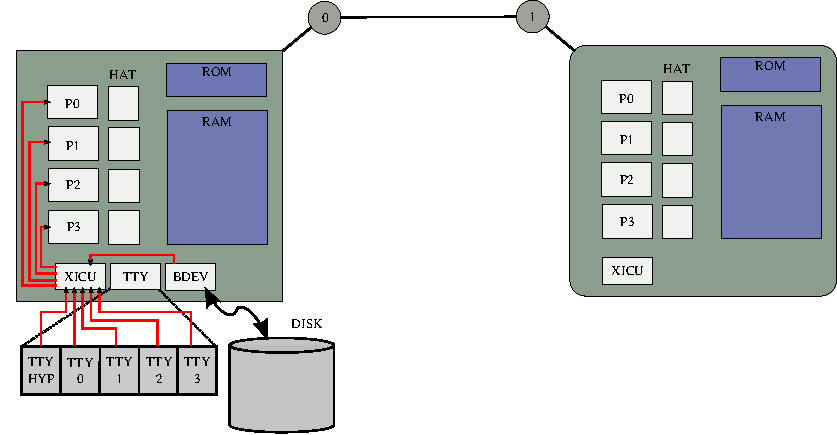
\includegraphics[width=8cm]{platform.pdf}
        \end{center}
\end{frame}

\section*{IOC}
\begin{frame}{IOC}
        \begin{center}
                \begin{block}{Problème}
                        \begin{itemize}
                                \item L'IOC n'a qu'une ligne d'interruption.
                                \item Un seul canal.
                        \end{itemize}
                \end{block}
                \pause
                \begin{block}{Solution}
                        \begin{itemize}
                                \item Ajout d'une ligne d'interruption vers toutes les XICUs de la plateforme
                                \item Un canal par cluster
                        \end{itemize}
                \end{block}
        \end{center}
\end{frame}

\section*{TTY}
\begin{frame}{TTY}
        \begin{center}
                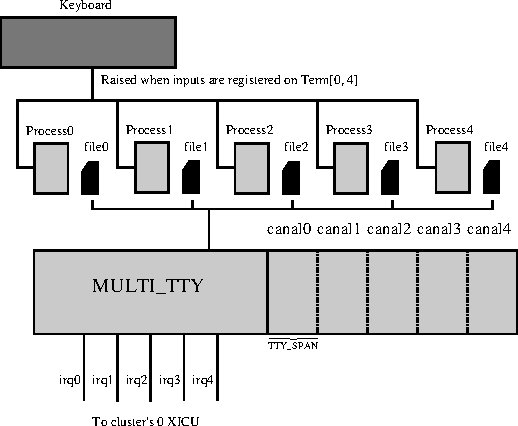
\includegraphics[width=9cm]{ttys_std.pdf}
        \end{center}
\end{frame}
\begin{frame}{Solution affichage TTY}
        \begin{center}
                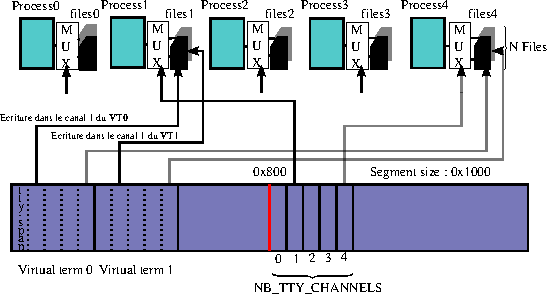
\includegraphics[width=10cm]{ttys_adv_w.pdf}
        \end{center}
\end{frame}

\begin{frame}{Solution interruptions TTY}
        \begin{center}
                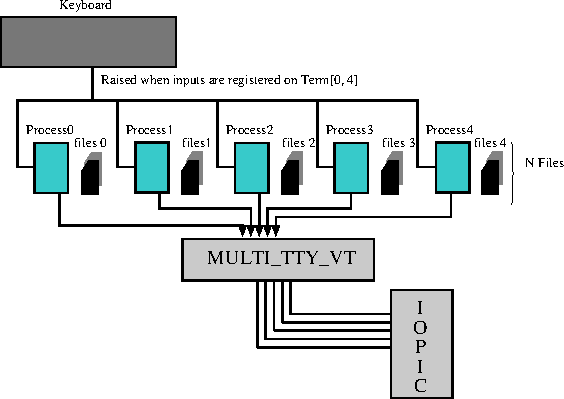
\includegraphics[width=10cm]{ttys_adv_r.pdf}
        \end{center}
\end{frame}

\section*{Lancement d'une VM}
\footnotesize
\begin{frame}{Lancement d'une VM}
        \begin{block}{Étapes}
                \begin{center}
                        \begin{itemize}
                                \item Allocation des canaux des périphériques, et des clusters
                                \item Construction de la structure décrivant l'architecture et copie
                                \item Lecture du bootloader et du kernel sur le disque et copie
                                \item Configuration des Hats (cloisonnement)
                                \item Réveil du processeur(IPI) en spécifiant l'adresse du bootloader
                        \end{itemize}
                \end{center}
        \end{block}
\end{frame}
\begin{frame}{Lancement d'une VM}
        \begin{block}{Étapes}
                \begin{center}
                        \begin{itemize}
                                \item Allocation des canaux des périphériques, et des clusters
                                \item Construction de la structure décrivant l'architecture et copie
                                \item Lecture du bootloader et du kernel sur le disque et copie
                                \item \textbf{Copie du code d'activation des Hats}
                                \item Réveil du processeur(IPI) en spécifiant l'adresse\textbf{ du code d'activation des Hats}
                                \item Configuration des Hats (cloisonnement) \textbf{par le proc 0 de l'instance}
                        \end{itemize}
                \end{center}
        \end{block}
\end{frame}
\normalsize
\begin{frame}
        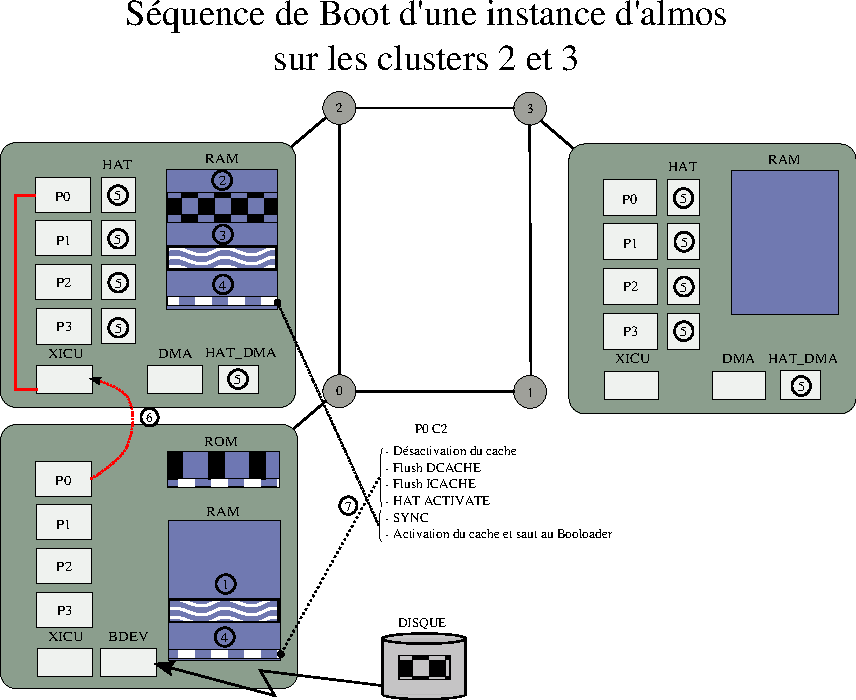
\includegraphics[width=10cm]{boot_23_simple.pdf}
\end{frame}






\end{document}



